% --------------------------------------------------------------------------- %
%                  _             _   _                                        %
%   _____   ____ _| |_   _  __ _| |_(_)_ __   __ _                            %
%  / _ \ \ / / _` | | | | |/ _` | __| | '_ \ / _` |                           %
% |  __/\ V / (_| | | |_| | (_| | |_| | | | | (_| |                           %
%  \___| \_/ \__,_|_|\__,_|\__,_|\__|_|_| |_|\__, |                           %
%                                            |___/                            %
%                                                    _            _           %
%                                        _ __   ___ | | __ _ _ __(_)___       %
%                                       | '_ \ / _ \| |/ _` | '__| / __| /\/| %
%                                       | |_) | (_) | | (_| | |  | \__ \|/\/  %
%                                       | .__/ \___/|_|\__,_|_|  |_|___/      %
%                                       |_|                                   %
% --------------------------------------------------------------------------- %
\chapter{Evaluating polaris\textasciitilde{}}\label{sec: polaris}
\begin{flushright}
    \Large\textsc{An Audiovisual Augmented Reality Experience Build on Open-Source Hardware and Software}
\end{flushright}
\begin{SingleSpace}
    \begin{tabular*}{\textwidth}{@{\extracolsep{\fill}}lr}
        \text{\faEdit}\quad\textbf{Blog:}&  \text{\url{https://www.sambilbow.com/projects/polaris}} \\
        \text{\faGithub}\quad\textbf{Code:}& \text{\url{https://www.github.com/sambilbow/polaris}} \\
        \text{\faListOl}\quad\textbf{Guide:}&  \text{\url{https://www.github.com/sambilbow/polaris/wiki}} \\
        \text{\faBook}\xspace\textbf{Publication:}&  \text{\url{https://dx.doi.org/10.21428/92fbeb44.8abb9ce6}} \\
        \text{\faFileArchiveO}\quad\textbf{Archive:}&  \text{\autoref{sec: appendix-b}}
    \end{tabular*}
\end{SingleSpace}%

\begin{figure}
    \centering
    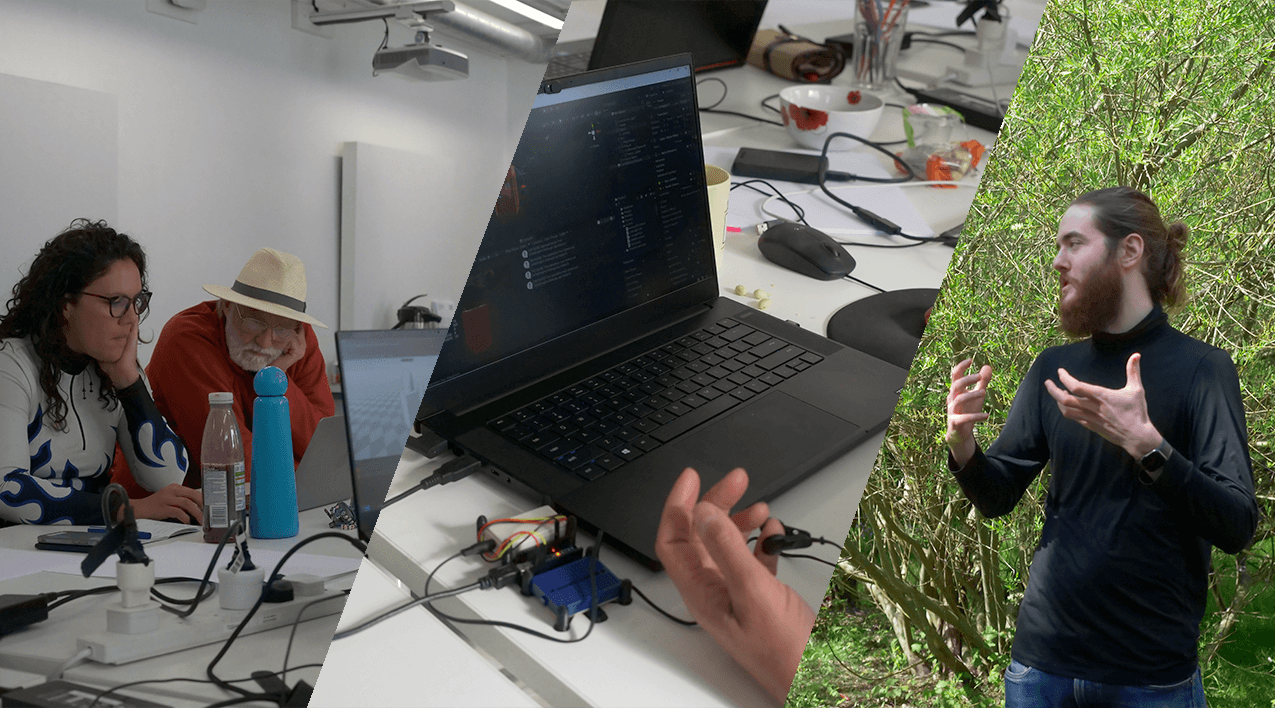
\includegraphics[width=1\linewidth]{06-polaris/chapter-fig.png}
    \captionsetup{labelformat=empty}
    \caption[\autoref*{sec: polaris}'s page-figure: Experience Study of \textit{polaris\textasciitilde{}} at the Sussex Humanities Lab (SHL), (from \citeauthor{bilbow2022}, \citeyear{bilbow2022})]{}
\end{figure}

    
\clearpage
   
% --------------------------------------------------------------------------- %
\section{Summary}\label{sec: polaris-summary}
This chapter outlines the development and evaluation of the \textit{polaris\textasciitilde{}} experience. \textit{polaris\textasciitilde{}} is built using a set of \glshyperlink[open-source]{opensource} \glshyperlink[hardware]{osh} and \glshyperlink[software]{floss} components that can be used to create privacy-respecting and cost-effective \gls{av} \gls{ar} experiences. Its wearable component is comprised of the \glshyperlink[open-source]{opensource} \gls{pns} \gls{ar} headset and a pair of bone conduction headphones, providing simultaneous real and virtual visual and auditory elements. These elements are spatially aligned using Unity and \gls{pd} to the real space that they appear in and can be gesturally interacted with in a way that fosters artistic and musical expression. In order to evaluate the \textit{polaris\textasciitilde{}}, 10 participants were recruited, who spent approximately 30 minutes each in the \gls{ar} scene and were interviewed about their experience. Using grounded theory, the author extracted coded remarks from the transcriptions of these studies, that were then sorted into the categories of Sentiment, Learning, Adoption, Expression, and Immersion. In evaluating \textit{polaris\textasciitilde{}} it was found that the experience engaged participants fruitfully, with many noting their ability to express themselves audiovisually in creative ways.

The objective of this chapter is to evaluate \textit{polaris\textasciitilde{}} as an \gls{ar} experience for its ability to provide a space for gestural \gls{av} expression, primarily through a user study, and later using the grounded theory method to extract relevant themes from participant interactions. The outcome of this research has contributed thoroughly to the design patterns in \autoref{sec: discussion-patterns}.


% --------------------------------------------------------------------------- %
\section{Designing \textit{polaris\textasciitilde{}}}\label{sec: polaris-framework}
The \textit{polaris\textasciitilde{}} experience itself is built using mostly \glshyperlink[open-source]{opensource} \glshyperlink[hardware]{osh} and \glshyperlink[software]{floss}. As well as creating the experience, I was interested in keeping a log of its framework in order to ensure its reproducibility and to facilitate further creation of a wide variety of \gls{av} \gls{ar} experiences. Any `artist-developer' \footnote{By using the term artist-developer, I refer to the media artist, creative coder, digital musician, or indeed any of the other many terms used to describe the category of artist who uses code and/or technology as their medium of artistic expression.} wanting to work on similar experiences should have the ability, when following this framework, to rapidly create and prototype low-cost and privacy-respecting sound \gls{art} experiences, and instruments..

\subsection{\textit{polaris\textasciitilde{}} Hardware}\label{sec: polaris-framework-hardware}
\subsubsection{Project North Star}\label{sec: polaris-framework-hardware-pns}

\begin{figure}
    \centering
    \subcaptionbox{Playing a virtual piano\label{fig: polaris-framework-hardware-pns-1}}{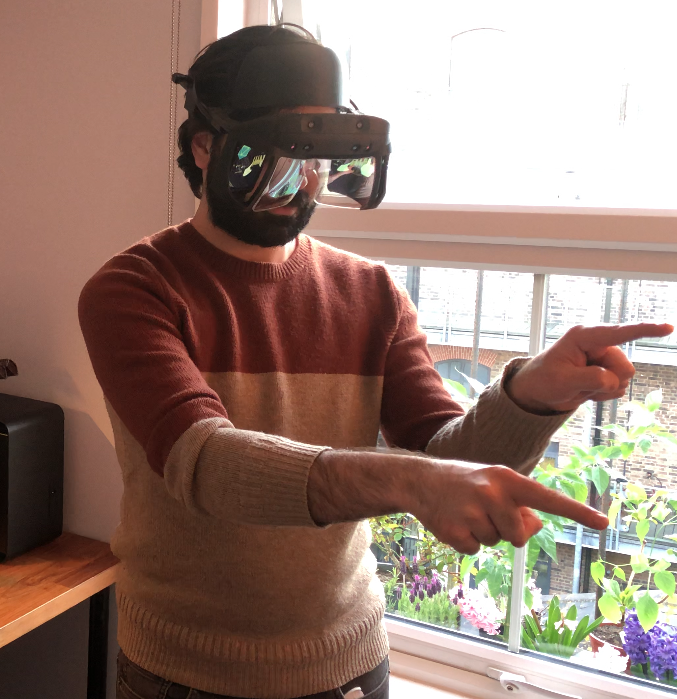
\includegraphics[height=4.5cm]{figures/06-polaris/polaris-framework-hardware-pns-1.png}}
    \hfill
    \subcaptionbox{Resizing and moving virtual objects\label{fig: polaris-framework-hardware-pns-2}}{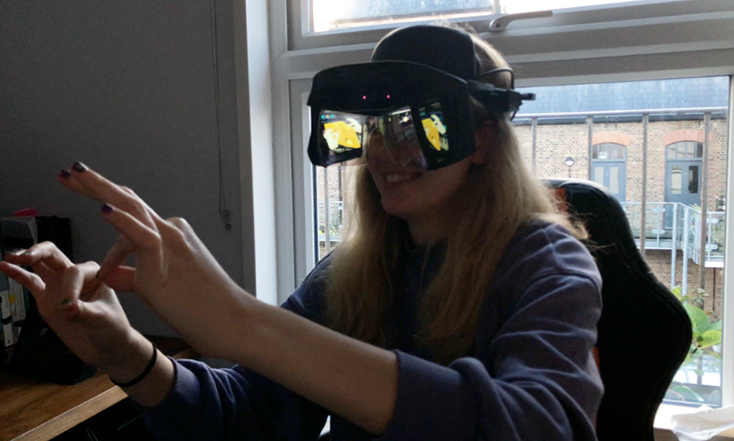
\includegraphics[height=4.5cm]{figures/06-polaris/polaris-framework-hardware-pns-2.png}}
    \caption{Project North Star in use during the prototyping phase of \textit{polaris\textasciitilde{}}}
\end{figure}

The primary section of wearable hardware is the \gls{pns} \gls{ar} headset, as \glshyperlink[open-source]{opensource}d by LeapMotion (now Ultraleap) in 2018. It has a 3D-printable assembly, and its circuit boards, cables, and screens are available to buy \href{https://docs.projectnorthstar.org}{online}; my \gls{pns} cost about \pounds500 in total to build - 5 to 6 times less expensive than the commercial \gls{ar} headsets mentioned, while maintaining industry-leading hand-tracking and \gls{6dof} tracking.

However, the time needed to build one and understand its workings well enough to trouble\-shoot any issues one faces may be a barrier to entry \footnote{I have found it a surprisingly integral part of the way I make sense of my creative practice, and fortunately there is a \gls{pns} Discord server with over 2400 helpful members that I have relied on heavily!}. Additionally, the finish material is not as polished as commercial headsets, and the overall size is larger and clunkier. It also needs to be tethered by USB and DisplayPort cable to a host computer or mobile compute pack.

\begin{wrapfigure}{r}{0.45\textwidth}
    \vspace{-\intextsep}
    \hfill
    \begin{minipage}{0.95\linewidth}
            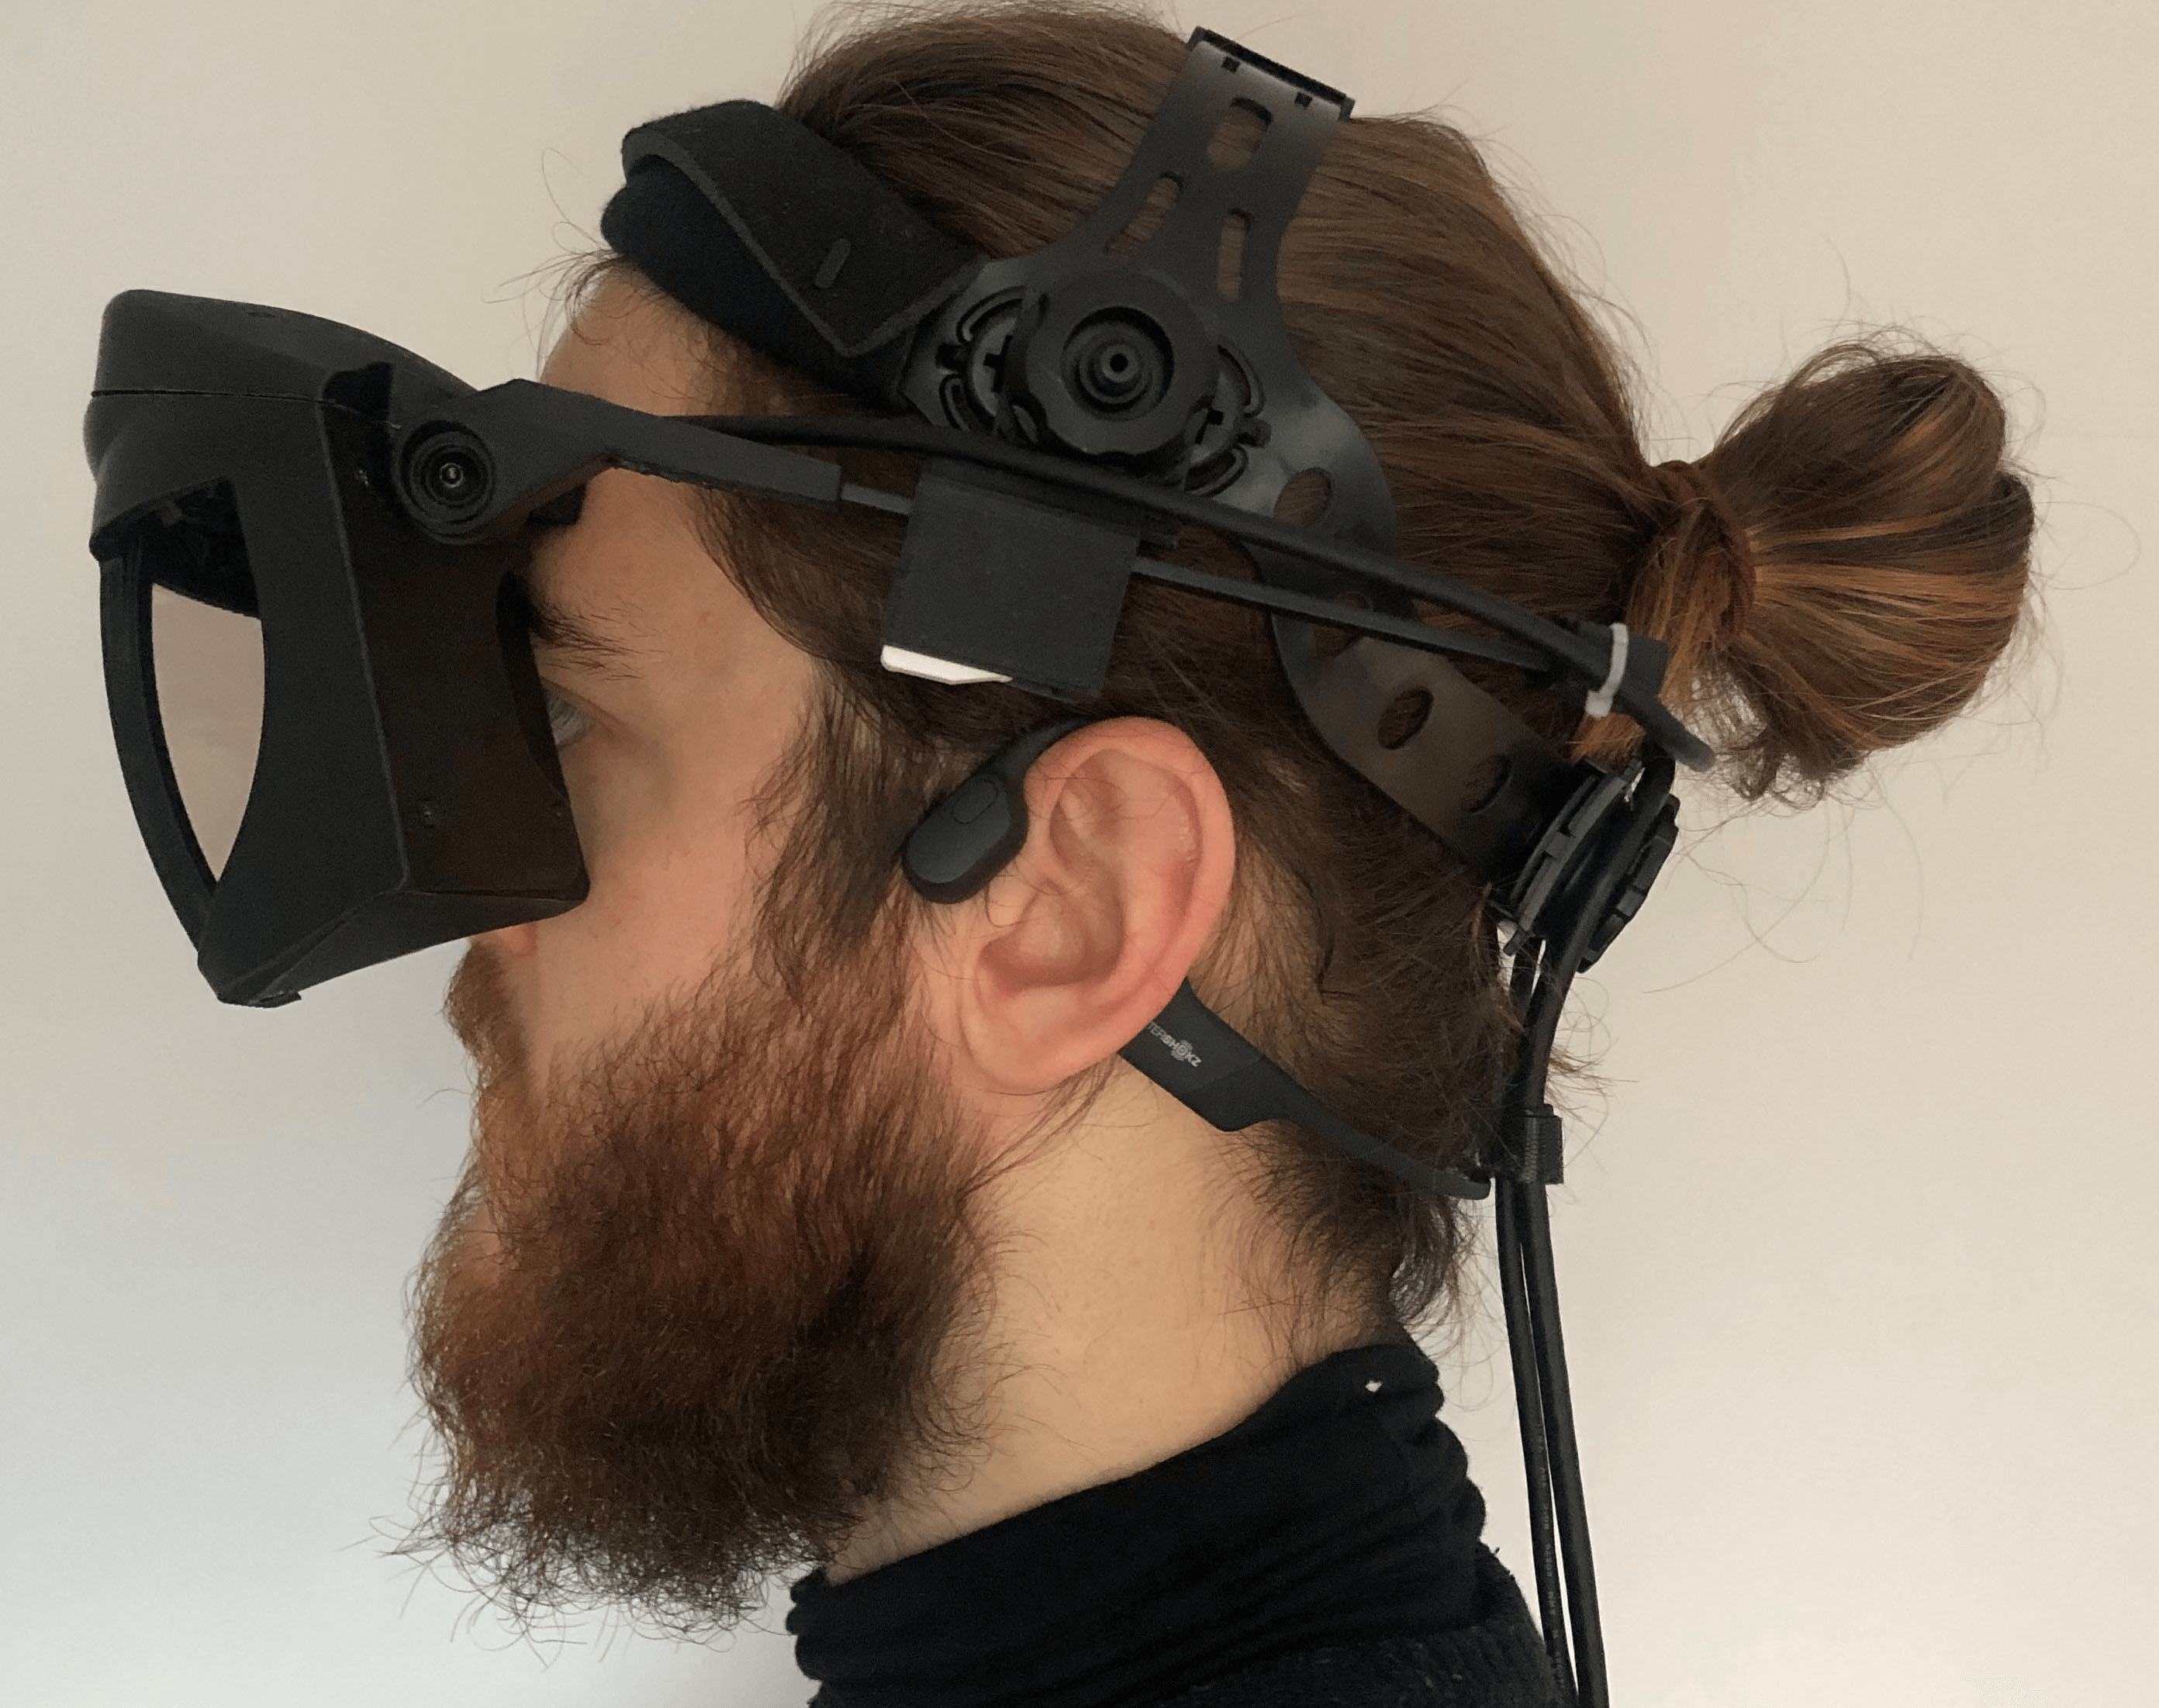
\includegraphics[width=\linewidth]{figures/06-polaris/polaris-framework-hardware-bc.png}
            \captionsetup{justification=justified}
            \caption{Project North Star worn with the addition of bone-conduction headphones}\label{fig: polaris-framework-hardware-bc}
    \end{minipage}
\end{wrapfigure}
Despite these drawbacks, my own experience of the headset has led to the rapid creation of many \gls{av} \gls{ar} prototypes. The fact that it requires no account to use, no developer's license to work with, and no data to be sent away to corporate servers has only added to my comfortability of using it as a creative tool.

\subsubsection{Bone Conduction}\label{sec: polaris-framework-hardware-bc}
The secondary piece of hardware in the system is a pair of bone-conduction headphones, seen in \autoref{fig: polaris-framework-hardware-bc}. These have been used as a method of auditory display in several other \gls{ar} projects \citep{lindeman2008,barde2016,chevalier2018}, typically for their ability to deliver audio in an unobtrusive fashion, as well as their comfortability and cleanliness in installation settings. They do not obscure the wearer's hearing of their real environment, making them suitable for emphasising the intertwined nature of virtual and real components of an \gls{ar} experience.


\subsection{\textit{polaris\textasciitilde{}} Software}\label{sec: polaris-framework-software}
\subsubsection{Unity}\label{sec: polaris-framework-software-unity}
\textit{polaris\textasciitilde{}} uses an \glshyperlink[open-source]{opensource} software companion to the \gls{pns} headset developed and maintained by Damien Rompapas \citeyearpar{rompapas2020}. At run-time, this Unity plugin (also making use of Ultraleap's Hands plugin) computes sensor readings from both the hand- and movement-tracking sensors and recreates the hand and headset pose in real-time inside the Unity scene. With the pose computed, it outputs the resultant view to the displays of the headset, rendering anything in the Unity scene relative to it.

Thanks to Unity's in-built audio spatialisation, any audio sample attached to an object in the Unity scene is, by default, spatialised in 3D and output via the bone-conduction headphones.

\subsubsection{Pure Data}\label{sec: polaris-framework-software-puredata}
In my own research, the desire to implement more than just sample-based audio interactions led me to experiment with many different options for implementing real-time audio synthesis. I ranked each option I found by its ability to fulfil the below criteria: (a write-up can be found on \href{https://sambilbow.github.io/projects/polaris/software.html}{my website}, or see \autoref{sec: appendix-b-blog-musical})

\begin{enumerate}
    \item Uses Unity's in-built audio spatialisation.
    \item Low computational cost on the host computer, and ability to be instantiated tens to hundreds of times procedurally.
    \item Ability to afford the artist-developer a wide palette of synthesis techniques.
    \item Allowing real-time parameter control of sounds via movement, gesture, and interaction with GameObjects in the Unity scene.
    \item Ability to rapidly prototype sound synthesis techniques and sonic interactions.
    \item Being free, \glshyperlink[open-source]{opensource}, and cross-platform.
\end{enumerate}

Meeting all these requirements was the \href{https://github.com/LibPdIntegration/LibPdIntegration}{LibPdIntegration} project developed and maintained by Niall Moody and Yann Seznec. It allows for the use of \gls{pd} patches in Unity, which, at run-time, are compiled to libPd (an embeddable version of \gls{pd}), and whose output is fed in real-time to the sound output of the GameObjects they are attached to  \footnote{The inclusion of \gls{pd} means that the many artist-developers can rely on a program that has existed in the field for nearly 25 years, many of whom will have experience using it.}.

To summarise, the use of the \gls{pns} companion software in conjunction with LibPdIntegration, allows for the creation of objects in an \gls{ar} scene that can have their own \gls{pd} patches. These can be parametrised to gesture, movement, and interaction, in ways that manipulate their audio synthesis in real-time and at low computational cost. This all while existing three-dimensionally in the participants' visual and auditory fields. The fact that this is delivered via an optical-see through headset and bone-conduction headphones results in an experience that does not significantly hinder (compared to \gls{vr}) the participants' ability to see and hear their real environment - augmenting and hybridising reality rather than replacing it.



% --------------------------------------------------------------------------- %
\section{Participant Studies}\label{sec: polaris-study}
In 2021, I ran a participant experience study of \textit{polaris\textasciitilde{}}, the first experience I created with the above framework. The main objective of the study was to extract (via grounded theory) participant sentiment towards their ability to audiovisually express themselves through gesture and movement in the \gls{ar} experience. Participants were recruited via university mailing-list, and were a mix of undergraduate and postgraduate Media, Film, and Music students.

\subsection{Questionnaire}\label{sec: polaris-study-questionnaire}
Participants completed a questionnaire, in which I asked for their age, gender identity, ethnicity, and occupation, to ensure a diverse and inclusive variety of participants. The mean age was \textasciitilde{}24.7 years old, with a range between 19 and 37; there were 6 female and 4 male participants, belonging to a diverse group of ethnicities.

\subsection{Tutorial}\label{sec: polaris-study-tutorial}
The participants were inducted into the experience via an introductory five-minute tutorial, the purpose being to ensure safety, build trust, and allow space for questions before beginning. This took the form of a narrated slideshow, in which I outlined the devices and interactions they should expect in the experience.

\subsection{The \textit{polaris\textasciitilde{}} Experience}\label{sec: polaris-study-experience}
Once the participant was wearing the headset and headphones, confirmed they were comfortable and they were standing in the starting position \footnote{As the headset was tethered to a computer, keeping the starting position the same between participants meant that the position of virtual content could be approximated to a clear space in the lab, marked by tape on the floor}, I began the Unity scene (a full demonstration of the scene can be found on my \href{https://youtu.be/lCBgMs8ULj0}{YouTube channel}), and let them know that the experience was about to start.

The experience involved nine floating iridescent `orbs', scattered at different distances from the starting position. The orbs would individually emit a repeating tone, whose pitch and tempo varied from orb to orb. Upon emitting a sound, the orb would eject a shower of white particles.

\begin{figure}[ht]
    \centering
    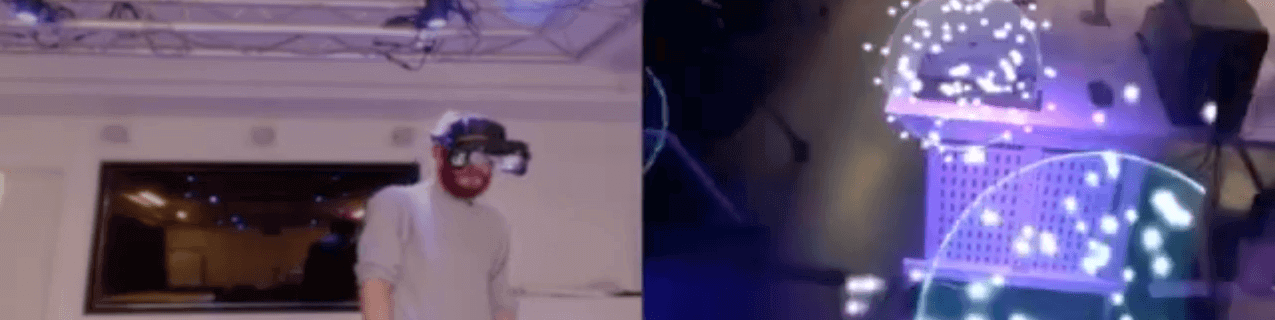
\includegraphics[width=.75\linewidth]{06-polaris/polaris-clip_1}
    \captionsetup{justification=centering,margin=1.5cm}
    \caption{Through-lens footage of the floating orbs in the polaris\textasciitilde{} AR scene \citep[from][\href{https://youtu.be/lCBgMs8ULj0?t=19}{at 00:19}]{bilbow2022c} \href{https://github.com/sambilbow/polaris/tree/main/unity/Assets/StreamingAssets/PdAssets/polaris_study_sphere}{(code)}}\label{fig: polaris-clip_1}
\end{figure}

Participants were invited to explore the space at their own pace. They could, of course, view the orbs from different angles, and hear their tones get louder and quieter as well as panning from ear to ear as they walked around them. I then prompted them to direct their gaze towards their hands, which were outlined, and when turning the left hand to face them, a menu appeared to the right of their palm. The menu contained two buttons, one labelled `Change Hand Colour', the other `Toggle Interactions'. I prompted them to tap the top button, which upon depressing slightly and providing an auditory `click', changed the colour of their hand's outline.

\begin{figure}[ht]
    \centering
    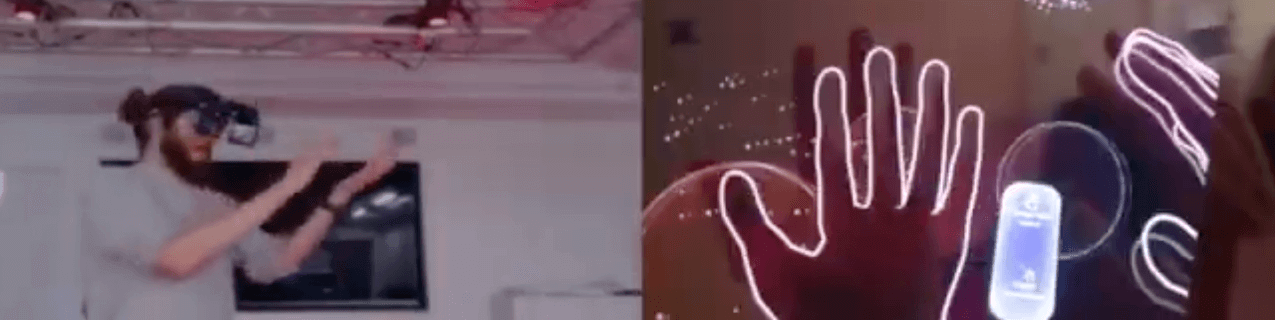
\includegraphics[width=.75\linewidth]{06-polaris/polaris-clip_2}
    \captionsetup{justification=centering,margin=1.5cm}
    \caption{Through-lens footage of the hand outline, menu, and button activation in the polaris\textasciitilde{} AR scene \citep[from][\href{https://youtu.be/lCBgMs8ULj0?t=140}{at 2:20}]{bilbow2022c}}\label{fig: polaris-clip_2}
\end{figure}

Upon toggling the second button on, constant streams of particles started emitting from the centre of their palms. These particles persisted for approximately five seconds to conserve computational power. While the button was toggled on, and the streams were emitting, each hand also produced a continuous noise \href{https://github.com/sambilbow/polaris/tree/main/unity/Assets/StreamingAssets/PdAssets}{(code)}.

In addition to these interactions, a total of five further interactions existed in the experience. The first two concerned the position, orientation, and gesture of the hands, relative to the participant. Firstly, they could modulate the depth of a vibrato effect on the sound of the particle stream by gradually turning their palms towards their face. Secondly, they could affect the sound's \gls{lpf} cut-off frequency by pinching their fingers together into a point, resulting in a hissing sound; paired with the visual feedback of narrowing the particle stream.

\begin{figure}[ht]
    \centering
    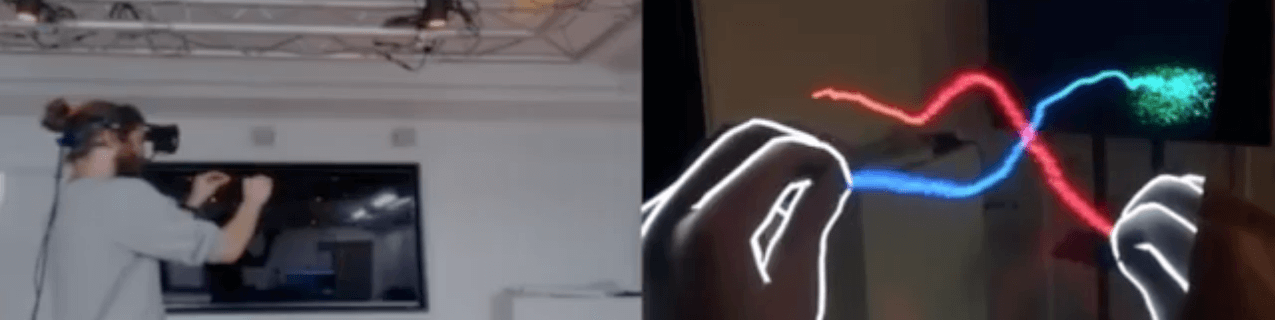
\includegraphics[width=.75\linewidth]{06-polaris/polaris-clip_3}
    \captionsetup{justification=centering,margin=1.5cm}
    \caption{Through-lens footage of the pinch gesture's effect on the particle streams in the polaris\textasciitilde{} AR scene \citep[from][\href{https://youtu.be/lCBgMs8ULj0?t=476}{at 7:56}]{bilbow2022c}}\label{fig: polaris-clip_3}
\end{figure}

On pointing their palms in the direction of an orb, the particles would gravitate towards the orb, and begin to slow down, orbit, and rotate it. Depending on which palm was pointing towards the orb, there would be an additional effect that increased in intensity as the participant persisted in pointing towards the orb. When pointing their left palm, over the course of 20 seconds, the orb's tone and white particle burst increased in tempo. When pointing their right palm towards an orb, over the course of 5 seconds, the depth of a tremolo effect on that orb's tone increased, with the paths of the white particles emitted from the orb becoming more erratic and corkscrew-like.

\begin{figure}[ht]
    \centering
    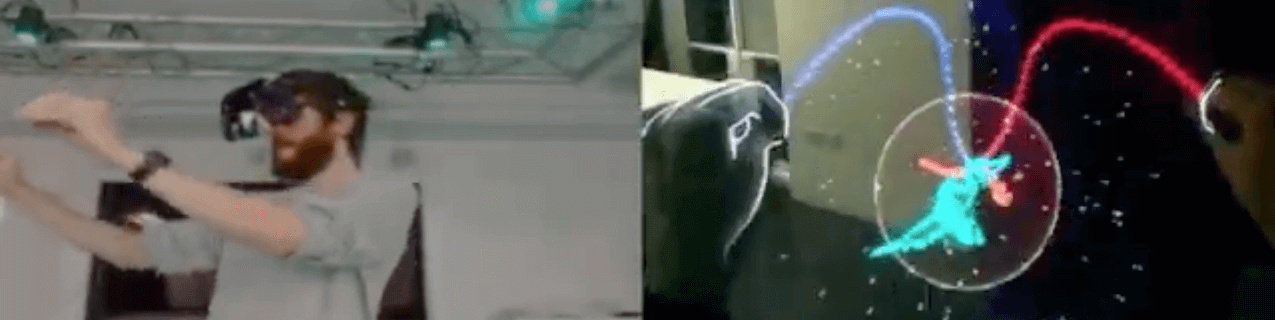
\includegraphics[width=.75\linewidth]{06-polaris/polaris-clip_4}
    \captionsetup{justification=centering,margin=1.5cm}
    \caption{Through-lens footage of the orb's gravitational effect on the hand particles in the polaris\textasciitilde{} AR scene \citep[from][\href{https://youtu.be/lCBgMs8ULj0?t=495}{at 8:14}]{bilbow2022c}}\label{fig: polaris-clip_4}
\end{figure}

Exploration of the scene differed between participants, but once they had either found or been shown the interaction methods in the scene and had either explored their variety or asked if there was anything else that they could do, I would ask them to try some experimental interactions.

Taking advantage of the vast number of parameters available to edit in Unity, I then changed elements of the visual   experience \footnote{Since the 11 \gls{pd} patches (9 for the orbs, and 1 each for the hands) were compiled at run-time they could not be edited on the fly} in real-time, asking for participant feedback on elements they preferred, and why. These elements of visual experience involved the orbs size, shape, gravity strength, and range; particle size, speed, lifetime, and colour.

\begin{figure}[ht]
    \centering
    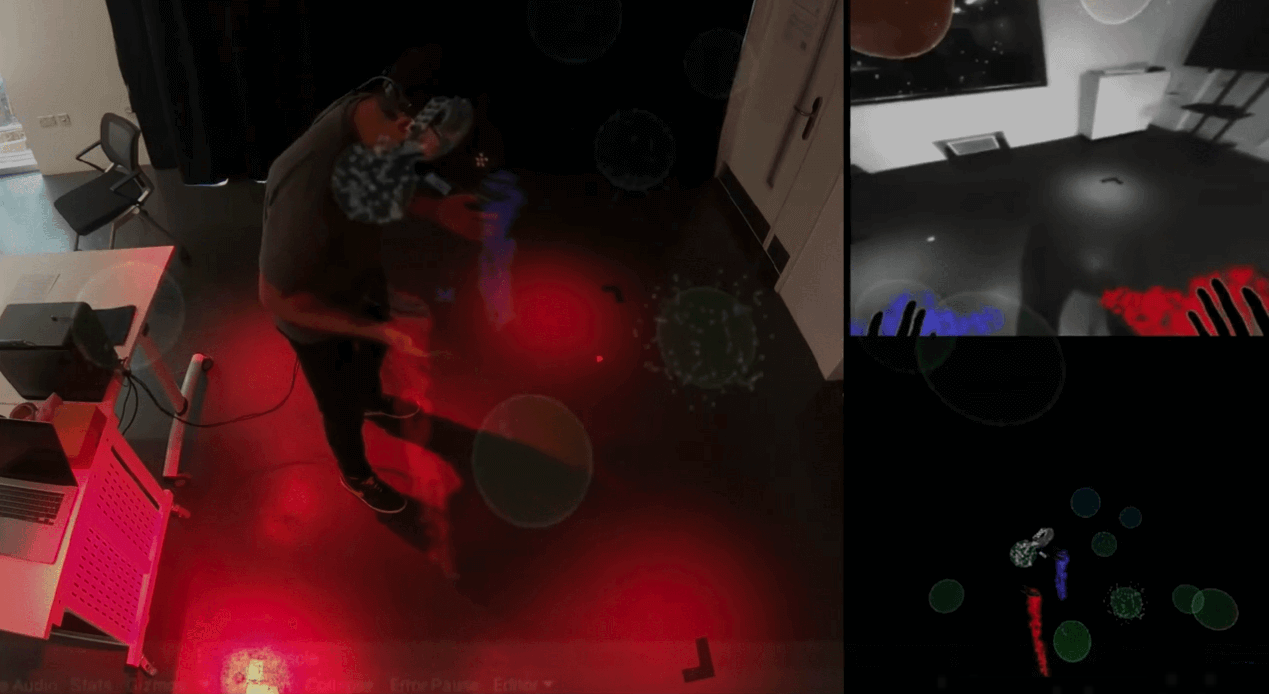
\includegraphics[width=\linewidth]{06-polaris/polaris-clip_5}
    \captionsetup{justification=centering,margin=1.5cm}
    \caption{Artificial composite 3rd and 1st person views of a polaris\textasciitilde{} participant drawing in mid air during the experimental section, note the scene gravity being turned on.  \citep[from][\href{https://youtu.be/72JLG1fGboY}{at 0:00}]{bilbow2022}}\label{fig: polaris-clip_5}
\end{figure}

\subsection{Interview}\label{sec: polaris-study-interview}
The next step of the study was a 10-minute interview, in which I asked participants about the positive and negative aspects of the experience, and anything they could suggest that would improve the experience. Questions were left deliberately broad due to the use of grounded theory to draw out themes for later analysis. I used a topic guide (see Appendix 1) to keep follow-on questions for replies related to the experience. This was in the form of a set of questions from the validated questionnaire titled `User Experience in Immersive Virtual Environments' by Katy Tcha-Tokey et al. \citeyearpar{tcha-tokey2016a}, which I adapted to suit \gls{ar}.

% --------------------------------------------------------------------------- %
\section{Results}\label{sec: polaris-feedback}
\subsection{Grounded Theory}\label{sec: polaris-feedback-grounded}
I chose the constructivist strand of grounded theory as developed by Kathy Charmaz \citeyearpar{charmaz2006} (building on the initial work by Glaser and Strauss \citeyearpar{glaser1967}) for my method of data analysis due to its ability to build theories from gathered data. Generally, generating a grounded theory extracts relevance from `codes' - line-by-line summaries of transcribed speech, that are then iteratively and repeatedly refined, and sorted into categories. This contrasts approaching data collection with a specific hypothesis in mind.

In the constructivist version of the Grounded Theory method, rather than assuming emergence of `unproblematic' and `objective' categories from the data itself, categories are admitted to being `mutually constructed' through interaction by the researcher with the data, considering and highlighting both the position and subjectivity of the researcher, as well as the partiality, and situational nature of the data itself.

In this instance, a study where I set out to evaluate the experience of participants in an \gls{av} \gls{ar} scene, I believed that it was suited to provide a rich set of data from which to critique and iterate the experience, and eventually build a set of \gls{msar} design guidelines.

\begin{figure}
    \centering
    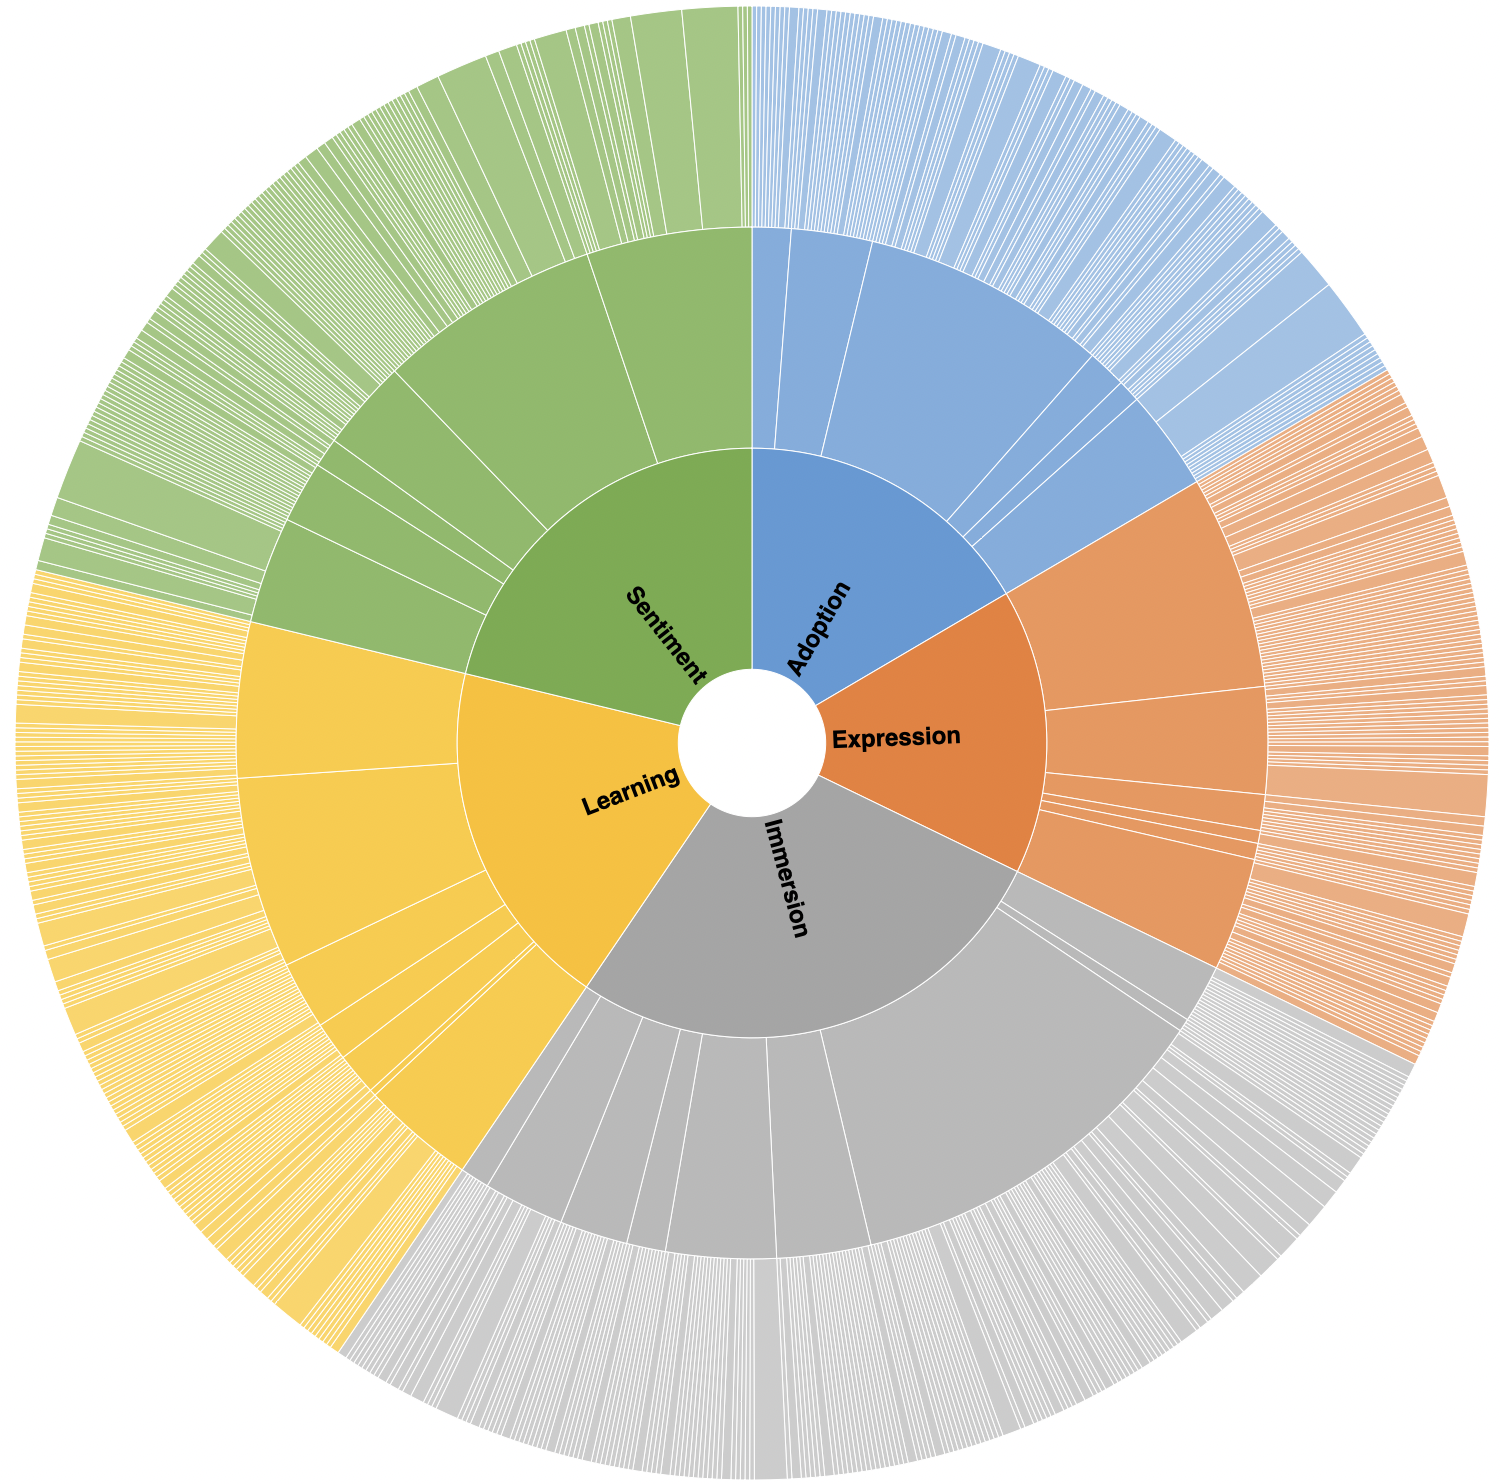
\includegraphics[width=0.7\linewidth]{figures/06-polaris/polaris-feedback-grounded-codes.png}
    \caption{5 categories, 37 subcategories and \textasciitilde{}700 codes visualised in NVivo.}
    \label{fig: polaris-feedback-grounded-codes}
\end{figure}

Transcribing the nearly 7 hours of experiences and interviews, lead to 45,858 words, and approximately \textasciitilde{}700 individual codes in the qualitative research software NVivo. These were sorted into 37 subcategories, with a total of 5 categories.

\subsection{Sentiment}\label{sec: polaris-feedback-sentiment}
Included in this category are emotions elicited by the experience, the majority of which were related to novelty. Participants felt a mixture of emotions, most frequently wonder or awe at the visual components of the scene, and enjoyment of the scene components and the interactions with them.

One participant felt fixated by the experience: \textit{`I am quite obsessed by this button'} (P9), whilst another felt satisfaction: \textit{`Like a fascination, wonder, it was quite satisfying as well'} (P3).

All participants made ample use of simile and metaphor, likening visual elements to liquid, snow, fire, fireworks, magic, and confetti. The sound design was said to be \textit{`ocean-like'} (P7) or \textit{`wind-like'} (P1), and participants expressed similarities in their experience to `being in' movies such as \textit{Star Wars, Minority Report, and Enter the Void} - \autoref{fig: films}.

\begin{figure}
    \centering
    \captionsetup{justification=centering, margin=1.5cm}
    \subcaptionbox{`The Force' \citep[from][]{kershner1980}\label{fig: kershner1980}}[.3\linewidth]{\includegraphics*[height=2.75cm]{06-polaris/kershner1980.png}}
    \hfill
    \subcaptionbox{Mid-Air Displays \citep[from][]{spielberg2002}\label{fig: spielberg2002}}[.3\linewidth]{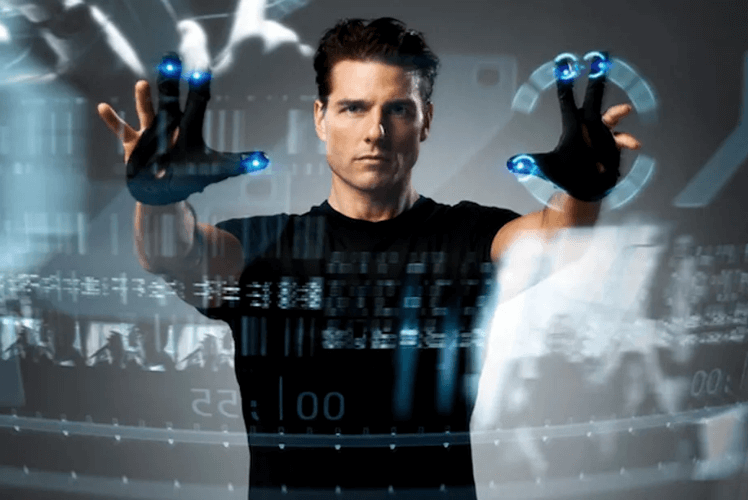
\includegraphics[height=2.75cm]{06-polaris/spielberg2002.png}}
    \hfill
    \subcaptionbox{Psychedelic Visuals \citep[from][]{noe2009}\label{fig: noe2009}}[.3\linewidth]{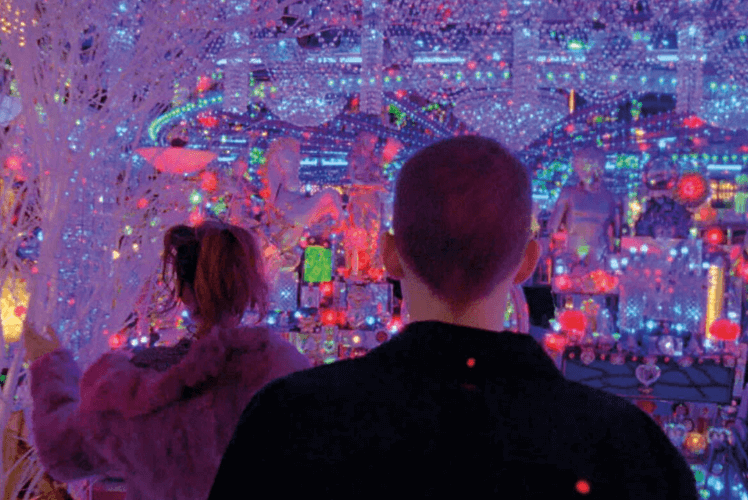
\includegraphics[height=2.75cm]{06-polaris/noe2009.png}}
    \caption{Participants likened the experience of \textit{polaris\textasciitilde{}} to `being in' \textit{Star Wars} \subref*{fig: kershner1980}, \textit{Minority Report} \subref*{fig: spielberg2002}, and \textit{Enter the Void} \subref*{fig: noe2009}}\label{fig: films}
\end{figure}

\subsection{Learning}\label{sec: polaris-feedback-learning}
From this category of codes, is clear that the experience involved an element of learning different functions and abilities. One participant remarked: \textit{`I was unsure, and I didn't know what would lead to a change in what I did, but after a point I understood'} (P6). Another linked learning as resulting in immersion: \textit{`Each step that you learn something new about what you can do in that environment, that's when you become more and more immersed'} (P9).

\subsection{Adoption}\label{sec: polaris-feedback-adoption}
This category includes codes that referred to issues that could be a barrier to using the technology, recommendations for different utilisations of \gls{av} \gls{ar}, and codes relating to safety and accessibility implications of adopting \gls{ar}.

\subsubsection{Comfort and Fit}\label{sec: polaris-feedback-adoption-comfort}
8 out of 10 participants struggled with the fit of the headgear on the \gls{pns} headset not being tight enough. As a result, some participants had to hold the headset with one hand throughout the experience. One participant expressed that this \textit{`stood as a hurdle to [the] experience'} (P1), and another specified how this affected their involvement with experience in more detail: \textit{`[Discomfort] doesn't ruin it, but it definitely brings me back to reality really quickly'} (P10).
\subsubsection{Alignment and Tracking}\label{sec: polaris-feedback-adoption-alignment}
Related to the above, were codes that referred to issues with alignment of content onto the real environment, such as the floating orbs and the outline of the hands. These were a product of the sensors, lighting, and content of the lab space. One participant even described the slight delay and misalignment of the hand outline as \textit{`trippy'} , going on to say that they \textit{`sort of like that it's a bit out'} (P1).

\subsubsection{Uses of AR and comparisons to other media}\label{sec: polaris-feedback-adoption-uses}
A wide variety of possible uses of \gls{av} \gls{ar} were highlighted by participants, including communication, conveying certain messages by highlighting important subject matter, art and music, virtual worlds, and video games.
One participant, who studies Media for Development and Social Change and works with environmental \glspl{ngo}, remarked that using \gls{av} \gls{ar} could help generate more interest in environmental conservation, because experiencing \gls{ar} made them feel \textit{`for some reason I act like this [virtual content] is more real than it is'}, going on to say that \textit{`rather than just watching it on the screen, you'd be more integrated'} (P6).

Another participant, studying on the same course, considered the use of \gls{ar} in the documentation of the lived experiences of vulnerable people, such as refugees. They emphasised that compared to traditional media formats, \gls{ar} was more \textit{`interactive'}, and that this could help in \textit{`angling the participant to be in touch with the subject more'} (P1), possibly helping raise awareness of vulnerable people without tokenising their lived experience.

Several other participants described the potential uses of \gls{ar} in artistic and musical contexts like \textit{polaris\textasciitilde{}}. One participant said that \gls{ar} had the potential to allow musicians to \textit{`easily feel'} and \textit{`play [...] with sounds'} (P2). One participant said that they could see \gls{ar} being used for both instrument-building and creating installations (P3).

\subsubsection{Safety and Accessibility}\label{sec: polaris-feedback-adoption-safety}
On the topic of safety, one participant expressed that despite \textit{`[feeling] like there will be lots of benefits for [the uptake of \gls{ar} and \gls{vr}]'}, they believed that it could lead people to \textit{`lose track of reality'} (P7). Overall, participants reacted positively to the fact that their concerns over the comfortability and fit of the headset would be able to be addressed thanks to the \glshyperlink[open-source]{opensource} nature of the \gls{pns}'s design.

\subsection{Expression}\label{sec: polaris-feedback-expression}
Participants expressed themselves in various ways during the \gls{ar} experience, and most described the ability to create visual and sonic components with their hands as the most compelling aspect of this expression. For example, one participant appreciated the variety of visual and sonic patterns that they could create: \textit{`when your hands are together, it made one style of shape, and when your hands were away it would make different styles that affected the music'} (P7), another emphasised variety as well as exploration: \textit{`[The experience] let me explore by using my hands [and] doing different gestures'} (P6).

\begin{figure}[ht]
    \centering
    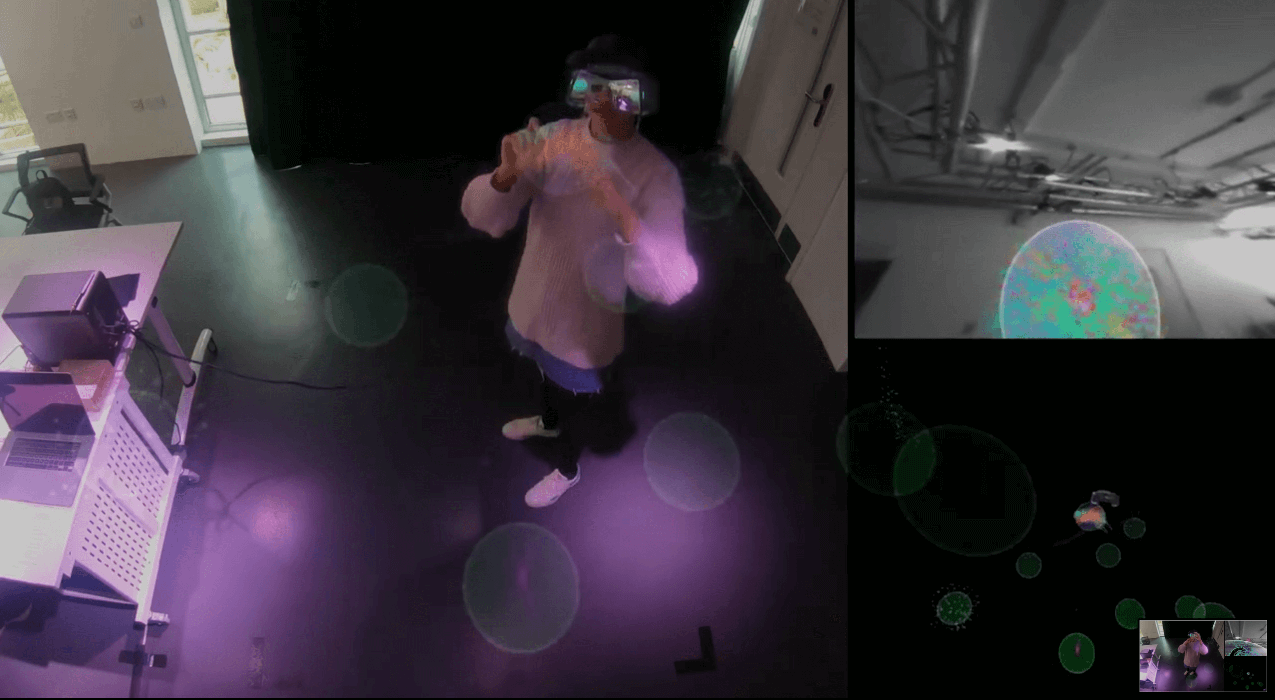
\includegraphics[width=\linewidth]{06-polaris/polaris-clip_6}
    \captionsetup{justification=centering,margin=1.5cm}
    \caption{Artificial composite 3rd and 1st person views of a polaris\textasciitilde{} participant using their hands to interact with the floating orbs \citep[from][\href{https://youtu.be/T7CAjPk2Zs0}{at 0:00}]{bilbow2022}}\label{fig: polaris-clip_6}
\end{figure}

Accordingly, several participants expressed their ability to act in the scene as \textit{`control'} or \textit{`power'}. One participant, almost sounding guilty, said: \textit{`I mean, it sounds weird, but I felt, like, very powerful'} (P10). Another, remarked similarly: \textit{`I think once I realised that I had the power to add things, I didn't let go of that'} (P3).

While one participant remarked that \textit{`physically doing something [that] you can see the effect of'} resulted in a feeling of \textit{`control'} (P7), another participant noted that they didn't always feel this: rather, that this might grow over time and with increased familiarity of the scene, reinforcing the suggestion of a learning process in the experience (P3).

Closely related to these codes were ones where participants expressed their wish to have more power and control over the scene, or that they had wished for different outcomes. Most common was the wish to be able to move the orbs around themselves (P3, 6, 9) or the ability to change elements as I had done in the experimental part of experience themselves, and at their own leisure (P5, 7, 9, 10).

One participant agreed that adding further visual indicators for the effects being had on the sound would help them notice these changes. The same participant commented that the pinching gesture used to tighten the stream of particles from the hand was unintuitive and would have preferred it to be a pointing gesture (P2).

\subsection{Immersion}\label{sec: polaris-feedback-immersion}
\subsubsection{Awareness}\label{sec: polaris-feedback-immersion-awareness}
Most participants reported that they felt aware of their real-world surroundings during the experience, one commenting that it was \textit{`because you could still see everything, you could still hear'} that they didn't get \textit{`lost'} in the experience (P7). However, one of the participants was adamant that they had \textit{`lost track of reality'} during the experience, and that it had felt \textit{`like [they were] in another environment'} (P9), another still, observing that there were moments when they forgot where they were (P10). It's clear then, that the experience immersed the participants, some more than others. When asked to offer a rationale for their feelings of immersion, participants pointed to several factors.

\subsubsection{Sights}\label{sec: polaris-feedback-immersion-sights}
One participant noted that they felt more immersed by the visual components of the scene, but that they would have felt less immersed if there wasn't an auditory component to the experience (P10). When being immersed by visual elements, for some it was colours that maintained this sense of immersion, with one participant commenting that the \textit{`vividness'} (P8) and size of the colours when particles had been made larger in the experimental section is what led to the moments of highest immersion in their experience.

\subsubsection{Sounds}\label{sec: polaris-feedback-immersion-sounds}
On the topic of immersion through audio, one participant put this down to the feeling of being \textit{`submerged'} in different layers of three-dimensional sound (P1). Similarly, many of the participants confirmed or independently reported to be able to discern and localise the tones they heard from different orbs around them, with some doing this by exploring through movement (P7), and others taking the visual cue of the white particle burst (P3). One participant remarked that the sound was the \textit{`main aspect'} of immersion for them, and that it made them \textit{`feel like part of'} the experience (P4); another commented that the sound \textit{`surrounded'} them and held their concentration so much that they almost forgot that they were wearing the bone-conduction headphones (P2). For another still, it was the activation of one of the orbs' sound effects that made them feel part of the experience (P3).

\subsubsection{Actions}\label{sec: polaris-feedback-immersion-actions}
A participant remarked that it was the feeling of \textit{`creating'} that led to their immersion. Additionally, they remarked that it was the \textit{`element of play'} in the interaction between particles and orbs that had immersed them in the experience; further noting that it was the way that the particles \textit{`emerged'} from their hands that kept them engrossed (P9). On playfulness and fun, another participant commented that it was the fact that they could interact with content that wasn't \textit{`there'} which was the most fun for them (P5).

\subsubsection{Physicality of Content}\label{sec: polaris-feedback-immersion-physicality}
One participant reported multiple times that they could \textit{`feel'} the button when they pressed it (although technically it was floating adjacent to their hand in mid-air). They agreed that it could be the mixture of the feedback sound, volumetric threshold trigger, and lighting that led to this effect (P9).

Another participant, upon placing their hands close to an orb remarked: \textit{`I know there's nothing there, but when I put my hand [towards the orb] I feel like I'm going towards something warm'}. This same participant expressed a keen interest during the experimental section in drawing large three-dimensional sculptures. During one of these drawings, the participant walked around their creation, and then took a moment before exclaiming: \textit{`Oh! I forgot that it wasn't a real thing, I kept trying to go [around] it, but I could just go through it!'}. Later, they noted: \textit{`I guess it's about our brains. [...] When we see it in 3D we automatically think it's more real than [if it were on a screen]'} (P8).

% --------------------------------------------------------------------------- %
\section{Conclusion}\label{sec: polaris-conclusion}
Overall, the \gls{ar} experience engaged participants fruitfully, with many noting their ability to express themselves audiovisually in creative ways. For \textit{polaris\textasciitilde{}}, the ability to do so whilst maintaining a privacy-respecting and cost-effective focus, is a testament to the individual components of the framework used to create it, and the labour that has facilitated the development of these \glshyperlink[open-source]{opensource} solutions.

The categories of codes extracted from the grounded theory analysis have resulted in a rich set of data. From those related to participant sentiment, it's not only clear that the \gls{av} \gls{ar} experiences are able to elicit a wide variety of emotions, but that to explain and make sense of them participants often made use of metaphors and past experiences. The fact that it was expressed multiple times by participants that the experience was one that they'd never had before might be a way of accounting for this variety and overlap of emotions.

Relating to the category of learning, it's clear that participants sensed this from multiple aspects of the experience, with one pointing towards the dimensionality, and others pointing towards the interactive elements and the need to explore the scene. For one participant there was a connection between learning and immersion. Within the context of musical interfaces, this could be taken to show that viewing the participant as a learner in the experience could lead to a deeper level of engagement.

Within the category of adoption, the fact that the headset lacked a good fit for most participants was clearly what detracted from the experience most. It led not only to a reduction in experience immersion, but also to a lessening of comfort and the knock-on effect of muscle fatigue and inability to exercise full agency for some participants. From the comments on different potential applications for \gls{ar}, it is clear that the offer of deeper interaction with subject matter, increased immersion in an experience, and the sense of \textit{`feeling'} or \textit{`playing'} with virtual content has led to participants envisaging \gls{ar}'s utilisation in several artistic and musical contexts. Notable was the suggestion that these facets of experience, especially that of the three-dimensional and context-specific sounds, could be employed to convey messages of socio-ethical importance as well as aesthetic experience. It is important to mention that some participants warned of negative side-effects or the potential for negative experiences in \gls{ar}, showing the importance for an inclusive and safety-minded approach to designing such \gls{ar} experiences.

To improve on the comfortability of the experience, the first changes I made were to design an alternate headgear section for the headset. Over the course of a day, I collaborated with another \gls{pns} community member on \href{https://github.com/AheadIO/Deck-X/tree/main/Deck_X/STL_files/Headgear/Welding_Headgear_Adaptor}{3D printable designs}, which were merged into the main repository, and that would allow the quick and easy substitution of the main headgear piece for a smaller one that was more accommodating of smaller head sizes.

From the codes relating to self-expression and control, participants appreciated the ability to interact with their bare hands, and felt that this was the main contributor to their expression in the scene. This, for some, led to a feeling of power, and for some, a feeling of control over elements of the scene. For others, the feeling of control wasn't entirely certain, with some noting that the scene had agency of its own. It is also conclusive from these codes that some participants desired more control over the scene, although implementing this would have to be done thoughtfully, without overloading the scene with content and parameters to change.

Immersion tended to stem from the fact that the elements of the experience: sights, sounds, and actions were spatialised in three dimensions. Participants enjoyed and felt immersed by the movement and colour of the visual elements and were able to discern and localise the source of different sounds in the experience; several noting that this element was the most immersive factor for them, whilst others preferred the visual elements. Others still, noted that the actions that they employed, gestural and movement-based are what immersed them in the experience most, and for some, this led to the virtual content of the scene feeling physical at times.

\begin{figure}[ht]
    \centering
    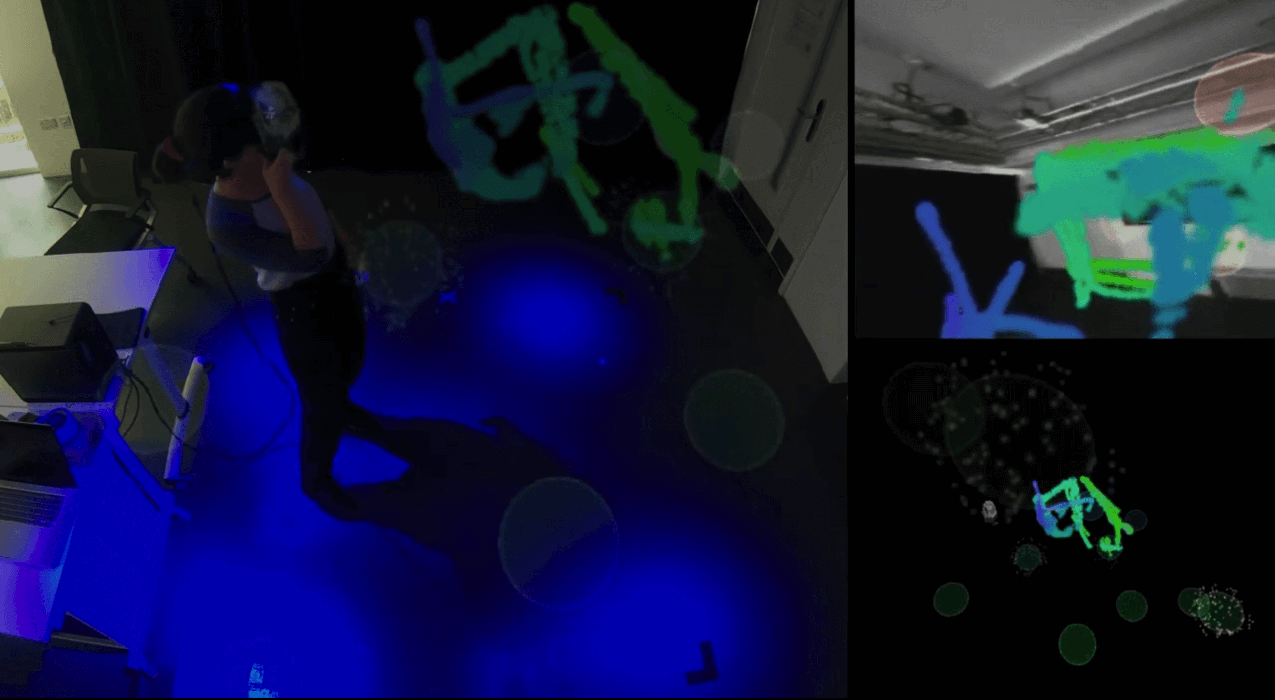
\includegraphics[width=\linewidth]{06-polaris/polaris-clip_7}
    \captionsetup{justification=centering,margin=1.5cm}
    \caption{Artificial composite 3rd and 1st person views of a polaris\textasciitilde{} participant expressing themselves in the scene, and viewing their creation from different angles \citep[from][\href{https://youtu.be/H8d3n7eNKAg}{at 0:00}]{bilbow2022}}\label{fig: polaris-clip_7}
\end{figure}    

While the above analysis is not, on its own, sufficient to draw conclusive guidelines for design, it does shed light on several connections between elements of this specific experience: learning, comfort, safety, spatial perception, visual-, sonic-, and action-led immersion, and physicality of virtual content. In \autoref{sec: discussion-medium} this is expanded upon, and this has lead to the iteration of parts of the design patterns found in \autoref{sec: discussion-patterns}.
